\newpage
\section{Clustering}
%\begin{figure}[H]
%  \centering
%  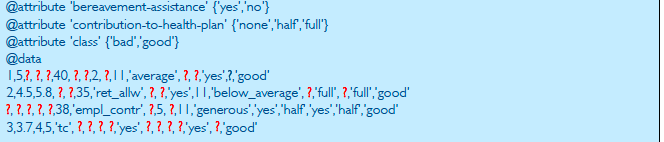
\includegraphics[width=.5\linewidth]{arffmissing}
%\end{figure}
\subsection{Intro}
Clustering is an \textbf{unsupervised} (no predefined class) machine learning technique that \textbf{groups} a collection of data point into \textbf{clusters} according to some \textbf{distance measure} so that data points in the cluster have \textbf{a small distance} from each other and data points in different clusters should be at large distances.\\
Good clustering consists of :
\begin{itemize}
\item High intra-class similarity
\item Low inter-class similarity
\end{itemize}
The quality of clustering depends on the \textbf{similarity measure} (but also by its \textbf{implementation}) and its ability to find some or all \textbf{hidden patterns}.
To evaluate the goodness of clustering :
\begin{itemize}
\item Various measures of similarity
\item Manual inspection
\item Benchmark with existing labels
\end{itemize}
The similarity is usually expressed as a function of \textbf{distance},typically metric $$ d(i,j)$$. This distance functions depend on the variables used , as they differ for interval-scaled,boolean, categorical ,ordinal ratio, and vector variables.  The \textbf{goodness} of clustering however must be measured by \textbf{another function}. The concept of \textbf{good enough} is very \textbf{subjective}!

\subsubsection{Clustering methods}
\begin{itemize}
\item Hierarchical vs point assignment
\item Numeric and/or symbolic data
\item Deterministic vs non deterministic
\item Exclusive vs overlapping
\item Hierarchical vs flat
\item Top-down vs bottom-up
\end{itemize}

\subsubsection{Data structures}
\begin{itemize}
\item \textbf{Data matrix}\\
$$ \begin{bmatrix}
 x_{11} & ... & x_{1f} & ... & x_{1p} \\
... & ... & ... & ... & ... \\
 x_{i1} & ... & x_{if} & ... & x_{ip} \\
 ... & ... & ... & ... & ... \\
  x_{n1} & ... & x_{nf} & ... & x_{np}
\end{bmatrix}
$$

\item \textbf{Dis/Similarity Matrix}\\
$$ \begin{bmatrix}
 0 &  &  &  & \\
 d(2,1) & 0 &  &  &  \\
 d(3,1) & d(3,2) & 0 &  &  \\
 ... & ... & ... & ... & ... \\
  d(n,1) & d(n,2) & ... & ... & 0
\end{bmatrix}
$$
\end{itemize}

\subsubsection{Distance and Similarity Measures}
The measures are very similar to the ones used in KNN:
\begin{itemize}
\item $L_r$ norm
\item Euclidean distance $(r=2)$
\item Manhattan distance $(r=1)$
\item $L_{\infty}$ norm
\item Jaccard distance
\item Cosine distance 
\item Hamming distance
\item Edit distance (new)\\
The distance between a string x=$x_1x_2...x_n$ and y =$y_1y_2...y_m$ is the \textbf{smallest number of insertions and deletion} of single character that \textbf{transform x into y} or can be defined as the \textbf{longest common subsequence LCS} of x and y and then $$ d(x,y) = |x| + |y| -2|LCS|$$  
\end{itemize}

\subsubsection{Requisites for clustering}
\begin{itemize}
\item Scalability 
\item Ability to deal with different types of attributes
\item Ability to handle data dynamically
\item Discovery of clusters dynamically
\item Discovery of clusters with arbitrary shape
\item Able to deal with \textbf{noise} and \textbf{outliers}
\item Incorporate user specified constraints
\item High dimensionality\\
\textbf{Curse of dimensionality}: in high dimensions ,almost all pair of points are \textbf{equally far away from one another} $\rightarrow$ \textbf{orthogonal vectors}
\item Insensitive to order of inputs
\item Interpretability and usability
\end{itemize}

\subsection{Hierarchical clustering}
One of the most common types of clustering. Can be done in two ways:
\begin{itemize}
\item \textbf{Agglomerative}\\
Start at \textbf{individual clusters}, at each step ,merge the \textbf{closest pair} of clusters until \textbf{one cluster} o \textbf{k-clusters} left
\item \textbf{Divisive}\\
Start with \textbf{one cluster} ,at each step , \textbf{split a cluster} until each cluster contains a point or there are k-clusters.
\end{itemize}
\begin{figure}[H]
  \centering
  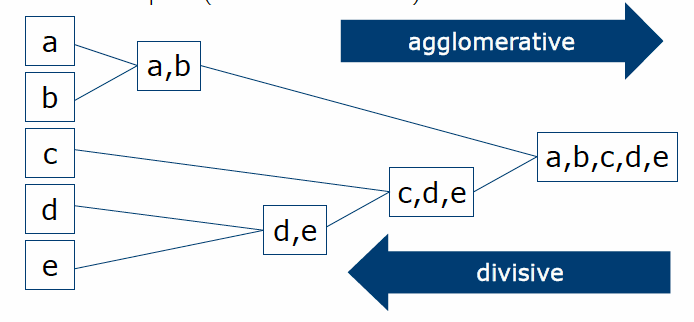
\includegraphics[width=.6\linewidth]{kclust}
\end{figure}
Easy to used and any desired number of cluster can be obtained by \textbf{cutting} the dendrogram at a proper level. Traditional hierarchical clustering algorithms use \textbf{similarity} or \textbf{distance matrix} to merge or split \textbf{one cluster at the time}.\\
The most popular is the \textbf{agglomerative} algorithm :
\begin{enumerate}
\item Compute proximity matrix
\item Let each data point be a cluster
\item Repeat until single cluster remains :
\begin{itemize}
\item Merge two \textbf{closest} clusters
\item \textbf{Update} proximity matrix
\end{itemize}
\end{enumerate}
Key operation is to define the \textbf{proximity} matrix between two clusters : different algorithm use different measures and lead to different clusters.

\subsubsection{Complexity}
\begin{itemize}
\item $O(N^2) $ space since it uses the \textbf{proximity matrix}
\item $O(N^3) $ in many cases : there are N steps at each step of size $N^2$ (proximity matrix must be searched and updated)
\end{itemize}
Efficient implementation :
\begin{itemize}
\item Compute distance between all points $O(N^2)$
\item Insert pairs and their distances in a \textbf{priority queue} to find the min one in one step $O(N^2)$
\item When merging two clusters, \textbf{remove all entries} in the queue involving one of these 2 clusters $O(NlogN)$
\item Compute the distance between the cluster and the remaining clusters $O(NlogN)$
\item Since the complexity of the \textbf{last two steps} is repeated \textbf{at most N times} ,total complexity is $$O(N^2 logN) $$
\end{itemize}

\subsubsection{Distance between clusters}
When merging two cluster who is the proximity matrix updated?
\begin{itemize}
\item \textbf{Single linkage or MIN}\\
\begin{figure}[H]
  \centering
  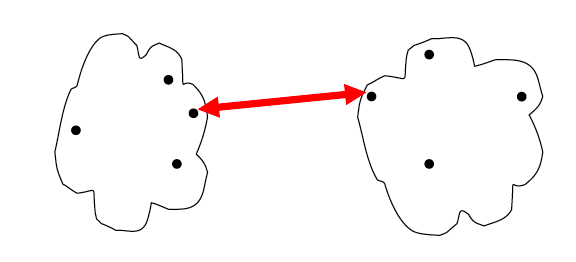
\includegraphics[width=.6\linewidth]{hgmin}
\end{figure}
Takes the \textbf{smallest distance} between an element of one cluster  and element in the other $$ d(C_i,C_j) = min (t_{i,p},t_{j,p})$$

\item \textbf{Complex linkage or MAX}\\
\begin{figure}[H]
  \centering
  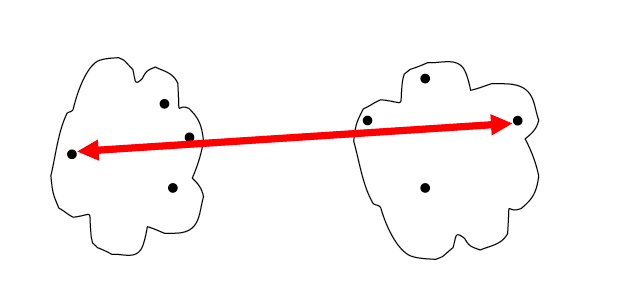
\includegraphics[width=.6\linewidth]{hgmax}
\end{figure}
Take the \textbf{largest distance} between an element in one cluster and an element in the other $$ d(C_i,C_j) = max (t_{i,p},t_{j,p})$$

\item \textbf{Average or Group Average}\\
\begin{figure}[H]
  \centering
  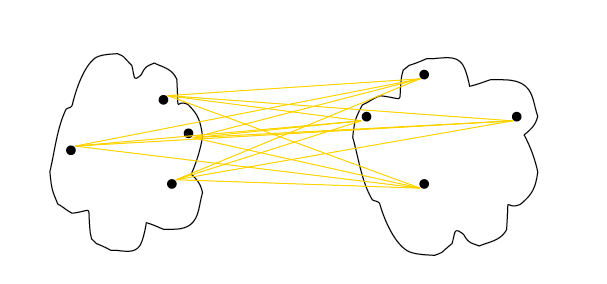
\includegraphics[width=.6\linewidth]{hgavg}
\end{figure}
Take the \textbf{average distance} between an element in one cluster and an element in the other $$ d(C_i,C_j) = avg (d(t_{i,p},t_{j,p}))$$

\item \textbf{Centroid}\\
\begin{figure}[H]
  \centering
  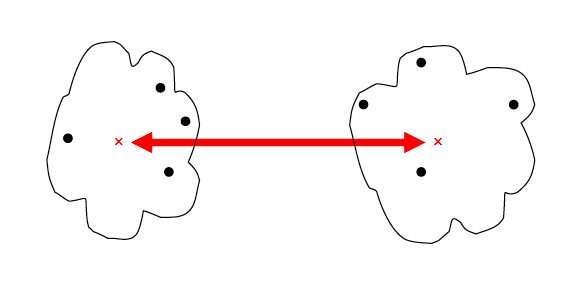
\includegraphics[width=.6\linewidth]{hgcentroid}
\end{figure}
Take the \textbf{largest distance} between an element in one cluster and an element in the other $$ d(C_i,C_j) = d(\mu_i , \mu_j)$$ where the $\mu$s are \textbf{centroids}
\end{itemize}

\subsubsection{Determining number of clusters}
HC generates a set of N possible partitions ,which one should be used?
A \textbf{good cluster} as already said should have small intra class distance and high inter class distance.\\
A good measure is the \textbf{Within/Between Cluster Sum of Squares}:
\begin{itemize}
\item \textbf{Within cluster SoS}:
$$ WSS(C) = \sum \limits_{I=1}^{k} \sum_{x_j \in C_i}|| x_j - \mu_i||^2 $$
where $\mu_i$ is the \textbf{centroid} of cluster $C_i$.\\
For a distance function \textbf{d}:
$$ WSS(C) = \sum \limits_{I=1}^{k} \sum_{x_j \in C_i}d( x_j - \mu_i)^2 $$

\item \textbf{Between-cluster SoS}:
$$ BSS(C) = \sum \limits_{i=1}^{K}|C_i|||\mu - \mu_i||^2$$
where $\mu$ is the centroid of the \textbf{whole dataset}.\\
For a distance function \textbf{d}:
$$ BSS(C) = \sum \limits_{i=1}^{K}|C_i|d(\mu - \mu_i)^2$$
\end{itemize}
Then a \textbf{knee/elbow analysis} is performed on the plots to show \textbf{significant} modifications in the evaluation metrics.

\subsubsection{Cluster representation}
In \textbf{Euclidean space} a cluster can be identified using for example its \textbf{centroid} or use its \textbf{convex hull}. In \textbf{Non-Euclidean} spaces a distance can be defined ( jaccard,cosine,edit) and the concept of \textbf{clusteroid} can be used : an \textbf{existing data point} used  as \textbf{representative} for the cluster ( can be the point that minimizes the sum of squares of the distances).
Another way to represent clusters if to check the \textbf{feature distribution} in the cluster and check if they are different.

\subsubsection{Problems with HC}
\begin{itemize}
\item Once a cluster merge has been done it cannot be undone
\item Sensitive to outliers and noise
\item No direct objective function to be minimized
\item Difficulty in breaking large clusters
\item Agglomerative method is commonly used by does not scale very well ( at least $O(N^2)$ complexity)
\end{itemize}

\subsection{Representative based Clustering}
The algorithms work around building the \textbf{representative} for each cluster .
Given a set of N instances and a desired number of k, this algorithms generate a partition C of N in k clusters :$$ \{C_i,...,C_k\}$$
And for each cluster there is a \textbf{point} that \textbf{summarizes} the cluster.
A common choice is to use the \textbf{mean} $$ \mu_i = \frac{1}{n_i} \sum \limits_{x_i \in C_i} x_i$$
with $\mu_i$ being the \textbf{centroid}.
The goal is to select the \textbf{best partition} according to some scoring function, for example the \textbf{sum of squared errors} :
$$ SSE(C) = \sum \limits_{I=1}^{k} \sum_{x_j \in C_i}|| x_j - \mu_i||^2 $$
$$ C^{*} = argmin_C SSE(C)$$
Brute force approach : $$ O(\frac{k^N}{k!} \text{ possible paritions}$$


\subsubsection{K-Means Clustering}
Most used representative based algorithm. It assumes an \textbf{euclidean} space can be easily extended to a non-euclidean case. The algorithm employs a \textbf{greedy} iterative approach that minimizes the SSE which can lead to find optimal solution but also often to sub-optimal solutions.
\begin{enumerate}
\item Choose k points that are likely to be in different clusters
\item Make these points the centroids of their clusters
\item For each remaining point : 
\begin{itemize}
\item find centroid to which the point is closest
\item add the point to the cluster
\item adjust centroid 
\end{itemize}
\end{enumerate}
\begin{figure}[H]
  \centering
  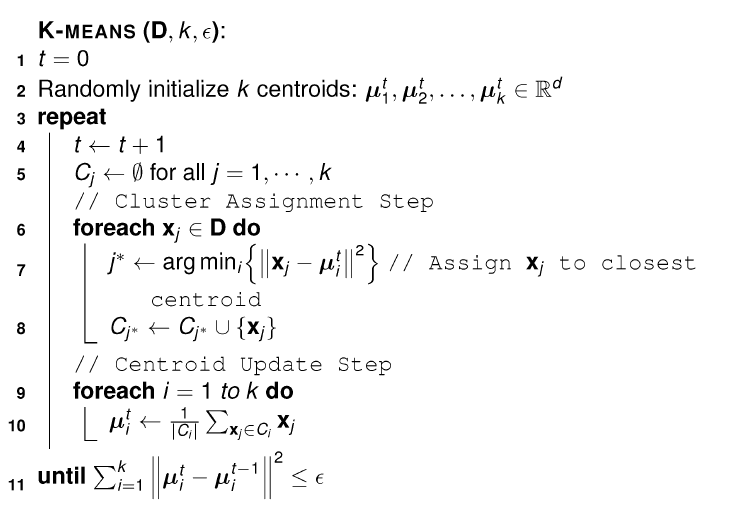
\includegraphics[width=.6\linewidth]{kmeans1}
\end{figure}

\begin{description}
\item{\textbf{Cluster initialization}}\\
The initialization of the clustering is important :
\begin{itemize}
\item \textbf{Solution 1}\\
Pick points that are as far away as possible from each other or pick the \textbf{first} point at random and while there are fewer than K points add the points whose \textbf{minimum distance} from the selected points is as \textbf{large as possible}.
\item \textbf{Solution 2}\\
Cluster a sample of data (hierarchically ?) so there are k-clusters. Pick a point from each cluster ( the one closest to the centroid?)
\end{itemize}
If there are K real clusters then the chance of selecting	 on centroid from each cluster is \textbf{small} (especially when K large).If clusters are the same size n:
$$ P \frac{\text{number of ways to select one centroid from each cluster}}{\text{number of ways to select K centroid}} = \frac{k!n^k}{(kn)^k}= \frac{K!}{K^k}
$$
So picking the right centroids is very hard and not always will they \textbf{converge} to the ideal centroid!\\
To overcome this issue:
\begin{itemize}
\item Multiple re-runs
\item Sample and use another sampling method
\item Select more than k-initial centroids and then select among these
\item Post-processing
\item \textbf{Bisecting k-means}\\
Can produce a partitional or hierarchical clustering 
\begin{figure}[H]
  \centering
  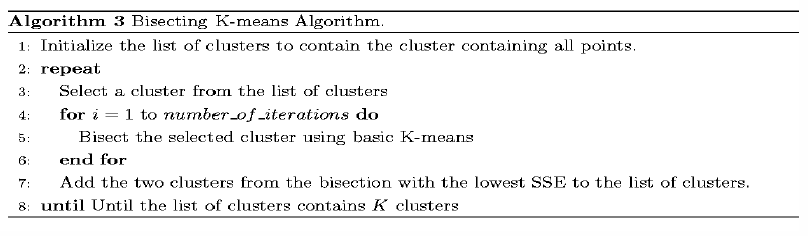
\includegraphics[width=.6\linewidth]{kmeans2}
\end{figure}

\end{itemize}

\item{\textbf{Cluster number}}\\
Also  the choice of the \textbf{number of clusters} must be made. A solution is to use the \textbf{Knee/Elbow Analysis}.

\item{\textbf{Centroid update}}\\
Centroid can be updated:
\begin{itemize}
\item When all points are assigned (usual method)
\item \textbf{Incrementally} , very expensive as each points updates zero or two centroids!
\end{itemize}
 
\item{\textbf{Pre and Post Processing}}
\begin{itemize}
\item \textbf{Pre-processing} : \textbf{normalize data} + \textbf{eliminate outliers}
\item \textbf{Post processing}: eliminate \textbf{small clusters}, \textbf{split} loose clusters ( relatively high SSE) , \textbf{merge} close clusters ( relatively low SSE)
\end{itemize}

\item{\textbf{Limitations of clustering}}\\
\begin{itemize}
\item \textbf{Differing Sizes}
 \begin{figure}[H]
  \centering
  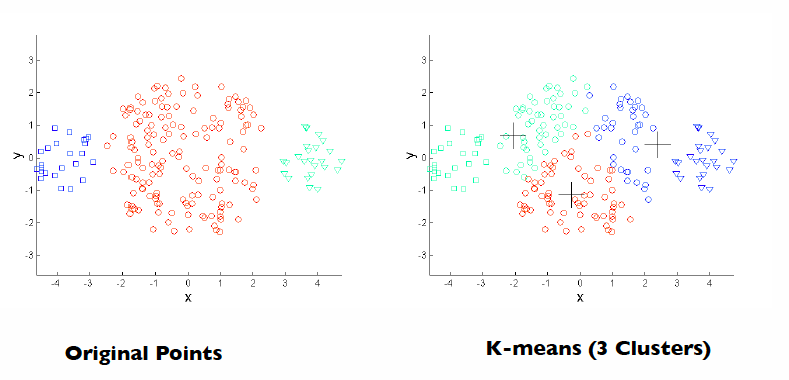
\includegraphics[width=.6\linewidth]{kmeans3}
\end{figure}
\item \textbf{Different densities}
\begin{figure}[H]
  \centering
  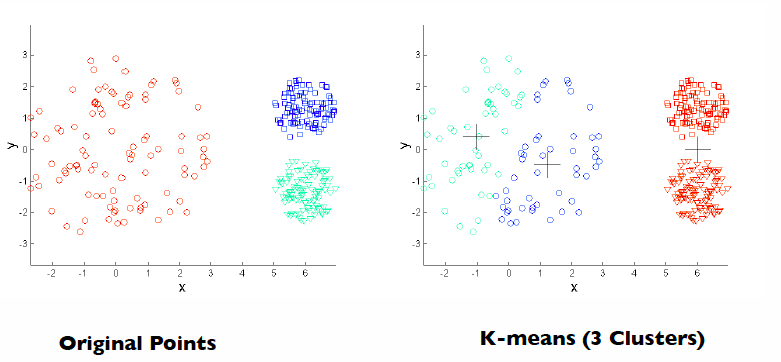
\includegraphics[width=.6\linewidth]{kmeans4}
\end{figure}

\item \textbf{Non globular shapes}
\begin{figure}[H]
  \centering
  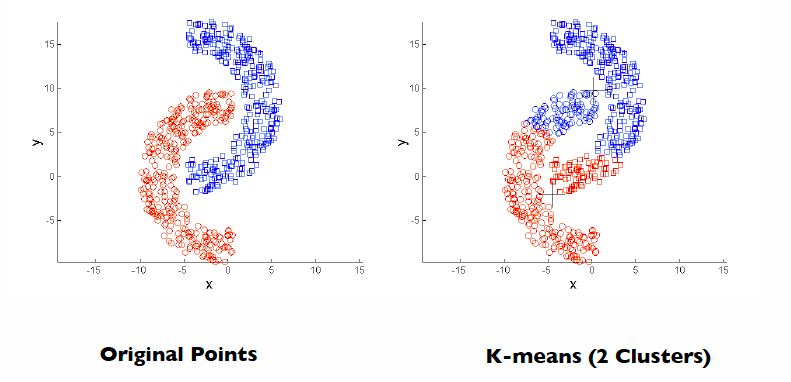
\includegraphics[width=.6\linewidth]{kmeans5}
\end{figure}
\end{itemize}
A solution to these can be to use \textbf{many clusters} and merge them (bigger k than expected).

\item \textbf{Summary}\\
\begin{itemize}
\item \textbf{Positive} :efficient , terminates often in optimal solution using annealing or genetic algorithms
\item \textbf{Negative} : only works when mean can be defined (no cat) , need to specify k in advance , bad with noisy data, not usable with cluster in non-convex shape
\end{itemize}
\end{description}

\subsubsection{BFR}
Extension to K-Means, can handle much more data (disk-resident data). It assumes that \textbf{data is normally distributed} around a \textbf{centroid}.Clusters are \textbf{axis-aligned ellipses}.\\
\begin{enumerate}
\item Points are read from disk one chunk at the time
\item Most points from previous memory loads are summarized by simple statistics
\item Select k initial centroids by sensible approach (k random points, take small sample and cluster optimally , take sample + random point then k-1 more points each as far away as possible)
\end{enumerate}
Points are divided into three sets: 
\begin{itemize}
\item \textbf{Discard set} = points close enough to a centroid to be summarized
\item \textbf{Compression set} = groups of points that are close together but not close to any existing point. These are \textbf{summarized} but \textbf{not assigned to a cluster}
\item \textbf{Retain set} = Isolated points waiting to be assigned to a compression set
\end{itemize}
\begin{figure}[H]
  \centering
  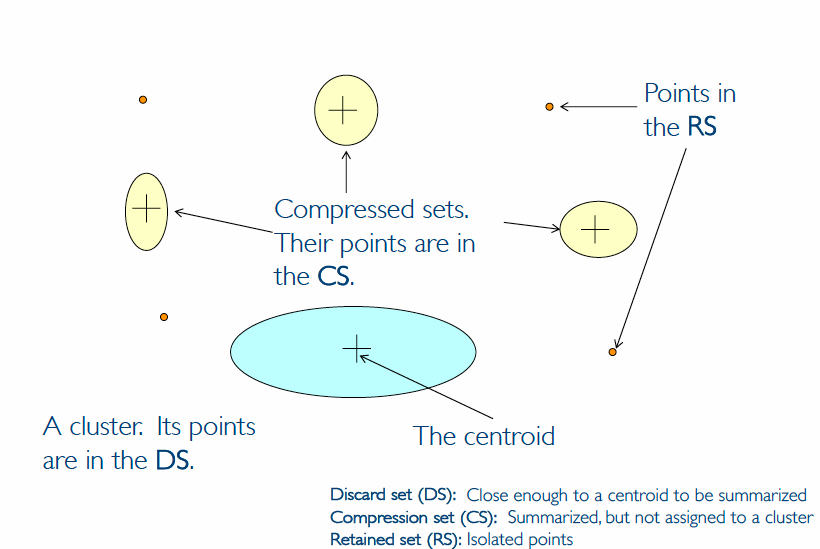
\includegraphics[width=.7\linewidth]{brf}
\end{figure}
The \textbf{discard set } is summarized by:
\begin{itemize}
\item \textbf{N} the number of points
\item \textbf{Vector SUM} whose component sum(i) is the sum of the coordinates of the points in the i-th dimension.
\item \textbf{Vector SUMQ} whose component sumq(i) is the sum of the square coordinates of the points in the i-th dimension.
\item 2 |dimension| + 1 represent the size of any cluster
\item Average in each dimension $\frac{SUM(i)}{N}$
\item Variance of cluster's discard set in dimension i $(\frac{SUMSQ(i)}{N})-(\frac{SUM(i)}{N})^2$
\end{itemize}
How the algorithm works :
\begin{enumerate}
\item First all points \textbf{sufficiently close} to the centroid of a cluster are added to that cluster (update points parameters) then discard the points

\item Points not close enough are clustered with the points in the \textbf{retain set} (can use any clustering algorithm)
\item Minicluster derived from new points + old retain set are merged
\item Any point outside a cluster is dropped 
\end{enumerate}
A point is \textbf{sufficiently close} then it is added using two approaches :
\begin{enumerate}
\item  Add p to cluster if it has the centroid closest to p and it is unlikely that after all points have been processed another centroid will be found closer to p
\item Measure probability that if p belongs to a cluster , it would be found as far as it is from the centroid of the cluster
\end{enumerate}
In practice the 	\textbf{Mahalanobis distance} is used :
it computes the distance between a point and the centroid of a cluster,normalized by the standard deviation of the cluster in each dimension
$$ \sqrt{\sum \limits_{i=1}^{d} \left( \frac{p_i-c_i}{\sigma_i} \right)^2}$$
A point is assigned to a cluster if \textbf{below a certain threshold}. For example threshold 4 means that there is a chance in a million not to include something that belongs to the cluster!\\

\subsubsection{Expectation Maximization}
K-means assigns each point to only one cluster \textbf{(hard assignment)}. Extend approach to consider \textbf{soft assignment} of points to clusters. Assume that each cluster $C_i$ is characterized by a multivariate \textbf{normal distribution} :
\begin{itemize}
\item mean vector $\mu_i$
\item covariance matrix $\Sigma_i$
\end{itemize}
Clustering is defined by a vector of parameters $\Theta$ :
$$ \Theta = \{ \mu_i \Sigma_i P(C_i) \}$$
The goal of MLE is to choose parameters so that :
$$ \Theta^{*} = argmax_{\theta} P(D|\Theta)$$
\begin{enumerate}
\item Start with initial estimate of vector parameter
\item Rescore the pattern against a mixture density produced by parameter vector
\item Rescored patterns used to update parameter vector
\item Patterns belonging to the same cluster, if they are placed by their scores in a particular component
\end{enumerate}
Maximize the probability that the data comes out of the found distribution :
\begin{figure}[H]
  \centering
  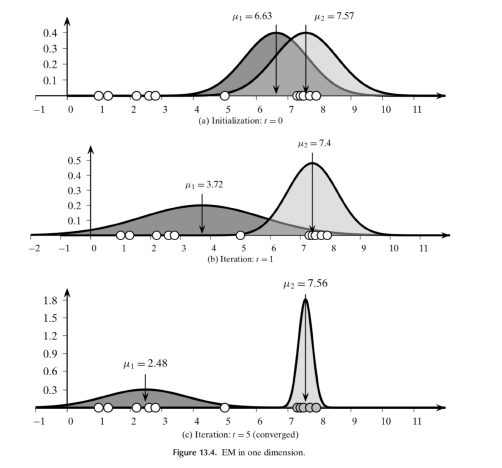
\includegraphics[width=.7\linewidth]{EM}
\end{figure}


\subsection{Density Based Clustering}
Density based clustering is a clustering technique based on density ,local cluster criterion , such as density connected points. It is useful as it can :
\begin{itemize}
\item Discover cluster of arbitrary shape (flexible)
\item Handle noisy data (robust)
\item Perform one scan (efficient)
\item Need density parameters as termination condition
\end{itemize}
Many interesting studies like \textbf{DBSCAN}:
\begin{itemize}
\item $\epsilon$ - neighbourhood of an object :
 $$ N_{\epsilon}(x) = \{ y | \delta(x,y) \leq \epsilon \}$$
 Is the neighbourhood with radius $\epsilon$ of a given object
\item \textbf{Core object} : if the $\epsilon$ - neighbourhood of an objects contains at least \textbf{minpts} then the object is a \textbf{core object}
\item \textbf{Directly density reachable} : an object x is directly density reachable from object y if x is within the $\epsilon$-neighbourhood of y and y is a core object
\item \textbf{Density reachable} : an object x is density reachable from y if there is a chain of object $x_1,...,x_n$ where $x_1=x$ and $x_n = y$ such that $x_{i+1}$ is directly reachable from $x_i$
\item \textbf{Density connected}: an object p is density-connected to q with respect to $\epsilon$ and MinPts if there is an object o such that both p and q are density reachable from o
\item \textbf{Density Based Cluster}: a density based cluster is defined as a maximal set of density connected points
\end{itemize}
\begin{figure}[H]
  \centering
  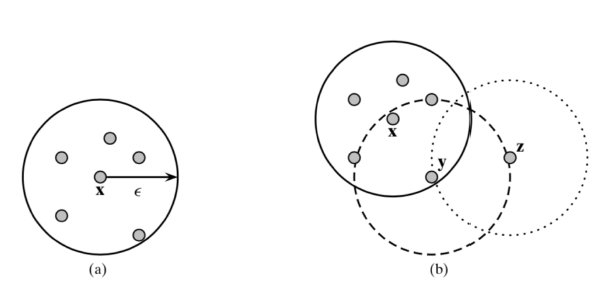
\includegraphics[width=.7\linewidth]{dbscan}
\end{figure}
\begin{itemize}
\item \textbf{Density} = have at least minpts within $\epsilon$
\item \textbf{Border} = fewer than minpts within $\epsilon$ but in neighbourhood of a \textbf{core point}
\item \textbf{Noisy} = is not a core point neither a border point
\end{itemize}
\begin{figure}[H]
  \centering
  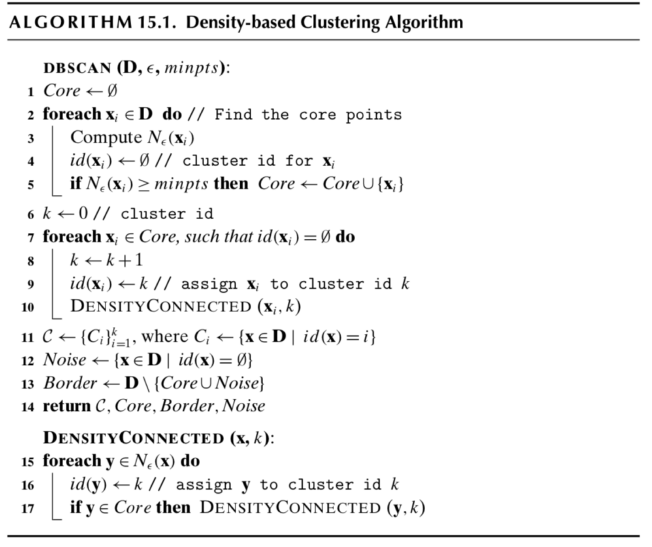
\includegraphics[width=.7\linewidth]{dbscan2}
\end{figure}
DBSCAN fails if the data:
\begin{itemize}
\item has \textbf{varying densities}
\item is \textbf{highly dimensional}
\end{itemize}


\subsection{Cluster Validation}
\subsubsection{Cluster Evaluation}
Cluster evaluation assesses the \textbf{goodness} or \textbf{quality} of the clustering.

\begin{description}
\item \textbf{1.External Validation Measures}\\
Employ criteria that are \textbf{not inherent} to the dataset (\textbf{prior} or \textbf{expert knowledge} about the clusters , like class labels for each point). Here the \textbf{ground-truth} is known a-priori.
\begin{enumerate}


\item \textbf{Using TP,FP,TN,FN}\\

\begin{itemize}
\item \textbf{TP} = number of true positive pairs. A pair $x_i,x_j$ are TP if they belong to the same \textbf{true partition T} and they are also in the \textbf{same cluster C}.
\item \textbf{FN} = number of false negative pairs.  A pair $x_i,x_j$ are FN if they belong to the same \textbf{true partition T} and they are also in the \textbf{same cluster C}.
\item \textbf{FP} = number of false positive pairs.  A pair $x_i,x_j$ are FP if they do not belong to the same \textbf{true partition T} but they are in the \textbf{same cluster C}.
\item \textbf{TN} = number of true negative pairs.  A pair $x_i,x_j$ are TN if they do not  belong to the same \textbf{true partition T} nor are they  in the \textbf{same cluster C}.
\item \textbf{N = TP+TN+FP+FN}
\end{itemize}

These measures allow to specify different \textbf{coefficients}:
\begin{itemize}

\item \textbf{Jaccard Coefficient} :  
$$\frac{TP}{TP+FP+FN}$$ , ignores the \textbf{true negatives}. Maximum value is \textbf{1} ( no FP , no FN).

\item \textbf{Rand Statistic} : 
$$\frac{TP+TN}{N}$$ ,measures all points were T and C agree.

\item \textbf{Fowlkes-Mallows Measure} : 
$$ \sqrt{\text{precision} \cdot \text{recall}}$$
$$\text{prec}= \frac{TP}{TP+FP} $$
$$ \text{rec}= \frac{TP}{TP+FN}$$
\end{itemize}

\begin{center}
\rule{0.8\textwidth}{.4pt}
\end{center}

\item \textbf{Mutual Information Based Scores}\\
Tries to quantify the amount of \textbf{shared information} between the clustering C and T $$I(C,T) = \sum \limits_{i=1}^{r} \sum \limits_{j=1}^{k} p_{i,j}log \left( \frac{p_{ij}}{p_{C_i} \cdot p_{T_j}} \right)$$
where $p_{ij}$ is the probability that a point belong to cluster i and ground-truth partition j , $p_{C_i} , p_{T_j}$ are the probabilities of cluster $C_i$ and partition $T_j$.\\
The \textbf{Normalized Mutual Information} score is :
$$ NMI(C,T) = \sqrt{\frac{I(C,T)}{H(C)} \cdot \frac{I(C,T)}{H(T)}} = \frac{I(C,T)}{\sqrt{H(C) \cdot H(T)}}$$ where $H_C = - \sum \limits_{i=1}^{r} p_{C_i} log p_{C_i} $ (same formula for H(T).\\
Values close to \textbf{0} indicate label assignments that are \textbf{largely independent} , close to \textbf{1} indicate \textbf{significant agreement}.

\begin{center}
\rule{0.8\textwidth}{.4pt}
\end{center}

\item \textbf{Homogeneity ,Completeness ,V-Measure}\\
\begin{itemize}
\item \textbf{Homogeneity} : each cluster contains only members of a \textbf{single class}
\item \textbf{Completeness}: all members of a given classa are assigned \textbf{to the same cluster}
\item \textbf{V-Measure}: \textbf{harmonic mean} of homogeneity and completeness
\end{itemize}
All between $[0,1]$ , the higher \textbf{the better}.
\end{enumerate}

\begin{center}
\rule{1\textwidth}{.1pt}
\rule{1\textwidth}{.1pt}
\end{center}

\item \textbf{2.Internal Validation Measures}
These are criteria derived from the \textbf{data itself}.These measures are based on the notion of \textbf{intracluster similarity} contrasted with the notion of \textbf{intercluster separation} : they usually provide a \textbf{trade-off} to maximize these two contrasting measures.
\begin{itemize}
\item Sum over all the \textbf{intracluster} weights over all the cluster 
$$ W_{in} = \frac{1}{2} \sum \limits_{i=1}^{k} W(C_i ,C_i)$$
\item Sum over all the \textbf{intercluster} weights 
$$ W_{out} = \sum \limits_{i=1}^{k-1} \sum \limits_{j>1}W(C_i,C_j)$$
\item Number of distinct \textbf{intracluster edges} $N_{in}$
 and \textbf{intercluster edges } $N_{out}$:
 $$ N_{in} = \sum \limits_{i=1}^{k} \binom{n_i}{2} = \frac{1}{2}\sum \limits_{i=1}^{k} n_i(n_i-1)$$
 $$ N_{out}= \sum \limits_{i=1}^{k-1} \sum \limits_{j>i}^{k} n_i \cdot n_j = \frac{1}{2} \sum \limits_{i=1}^{k} \sum \limits_{j \neq i, j=1}^{k} n_i \cdot n_j$$
 
\item \textbf{BetaCV}\\
Ratio of mean of intracluster distance to the mean of intercluster distance
$$ \text{BetaCV} =  \frac{W_{in} / N_{in}}{W_{out} / N_{out}}=  \frac{N_{out} \sum \limits_{i=1}^{k} W(C_i,C_i)}{N_{in} \sum \limits_{i=1}^{k} W(C_i,\bar{C_i})}$$
 The smaller this ratio \textbf{the better} : it indicates that on average the intracluster distances \textbf{are smaller} than intercluster distance
 
 \item \textbf{C-Index}\\
 Let $W_{min}(N_{in})$ be the sum of the \textbf{smallest} $N_{in}$ distances in the proximity matrix W , where $N_{in}$ is the total number of intracluster edges. Let $W_{max}(N_{in})$ be the sum of the \textbf{largest} distances in W. The \textbf{C-Index} measures to what extend the clustering puts together the $N_{in}$ points that are closest to the k clusters 
 $$C-index = \frac{W_{in}-W_{min}(N_{in})}{W_{max}(N_{in})-W_{min}(N_{in})} $$
 The \textbf{smaller} the \textbf{better} : indicates more compact clusters with relatively smaller distances within clusters rather than \textbf{between clusters}.

\item \textbf{Dunn-Index}\\
Ratio between minimum distance between points pairs from different clusters and the maximum distance between point pairs from same cluster
$$ \text{Dunn} = \frac{W^{min}_{out}}{W^{max}_{in}}$$
The \textbf{larger} the \textbf{better}: indicates that even the closest distance between points of different clusters is \textbf{much larger} than the farthest distance within same cluster.

\item \textbf{Davies-Bouldin Index}\\
The cluster mean is $\mu_i$ .The dispersion around the mean 
$$\sigma_{\mu}= \sqrt{\frac{\sum \limits_{x_j \in C_i} \delta(x_j,\mu_i)^2}{n_i}} = \sqrt{var(C_i)}$$
The measure , for a pair of cluster i and j, is:
$$ DB_{ij} = \frac{\sigma_{\mu_i}+\sigma_{\mu_j}}{\delta(\mu_i,\mu_j)} $$
This measure checks how \textbf{compact} the cluster is with respect to the \textbf{ distance between the cluster means}.\\
The index is finally defined as :
$$ \text{DB-Index } =\frac{1}{k} \sum \limits_{i=1}^k max_{j \neq i} \{ DB_{ij}\}$$
For each cluster i the cluster j is picked that \textbf{yields the largest DB ratio}.\\
The \textbf{smaller} the better: indicates that clusters are \textbf{well separated} and each cluster is well represented by its mean.


\item \textbf{Silhouette Coefficient}\\
Measures both cohesion and separation of clusters ,based on the difference between the average distance points int the closest cluster and to points in the same cluster
$$ s_i = \frac{\mu_{out}^{min} (x_i) - \mu_{in}(x_i)}{max \{ \mu_{out}^{min},\mu_{in}(x_i) \}}$$ 
where 
$$ \mu_{in}= \frac{\sum \limits_{x_j \in C_{\hat{y}}, i \neq j} \delta(x_i,x_j)}{n_{\hat{y}_i}-1}$$
$$ \mu_{out}^{in} (x_i)= min_{j \neq \hat{y}_i} \left\{ \frac{\sum \limits_{y \in C_j} \delta(x_i,y)}{n_j} \right\}$$
The values of $s_i$ lies between $[-1,+1]$:\\
- close to \textbf{1} : $x_i$ is much closer to points in its own cluster and far from other\\
- close to \textbf{0} : close to boundary between two clusters\\
- close to \textbf{-1} : $x_i$ is much closer to another cluster than to its own\\
The silouhette coefficient is defined as:
$$ SC =\frac{1}{n} \sum \limits_{i=1}^k s_i$$
The \textbf{closer} to \textbf{1} the \textbf{better}.\\
This measure should be used for convex clusters and not for DBSCAN for example

\item \textbf{Calisinki-Harabaz Index}\\
Given k-clusters CH-score s is given by the ratio of the \textbf{between cluster dispersion mean} and the \textbf{within cluster dispersion mean}:
$$ C = \frac{BSS(C) / (k-1)}{WSS(C) / (N-k)}= \frac{(N-k)BSS(C)}{(k-1)WSS(C)}$$
The \textbf{higher} the \textbf{better} : indicates that clusters are well separated.\\
The score is higher for convex cluster and lower for density based clusters.
\end{itemize}

\begin{center}
\rule{1\textwidth}{.1pt}
\rule{1\textwidth}{.1pt}
\end{center}

\item \textbf{3.Relative Measures}\\
Compare different clusterings obtained by varying different parameters for the same algorithm (e.g. number of clusters k).
\begin{itemize}
\item Knee/Elbow Analysis
\item Calisinki-Harabaz Index\\
Can be used to tare k : 
$$ \delta(k) = (CH(k+1)-CH(k)) - (CH(k)-CH(k-1))$$
\item Silhouette Coefficient\\
$s_i$ can be used to of each point $x_i$ and the average SC to estimate the number of clusters in the data : for each cluster plot $s_i$ values in \textbf{descending order}
\end{itemize}
\end{description}

\subsubsection{Cluster Stability}
Clusterings obtained from \textbf{several datasets} sampled from the same distribution should be \textbf{similar} or \textbf{stable}

\subsubsection{Cluster Tendency}
Aims to determine whether the dataset has any \textbf{meaningful groups to begin with}.Difficult task, tackled by comparing the data distribution with samples randomly generated from the same data space. Existing approaches use \textbf{spatial histograms}, \textbf{distance distribution}, \textbf{Hopkins statistic}